\documentclass{beamer}

\mode<presentation>
{
  \usetheme{Darmstadt}
  \setbeamercovered{transparent}
  \usecolortheme{default}
  \usefonttheme{default}
  \setbeamertemplate{navigation symbols}{}
  \setbeamertemplate{caption}[numbered]
}

\usepackage[english]{babel}
\usepackage[utf8]{inputenc}
\usepackage{listings}

\lstdefinestyle{customc}{
  belowcaptionskip=1\baselineskip,
  breaklines=false,
  xleftmargin=\leftmargini,
  language=C,
  showstringspaces=false,
  basicstyle=\ttfamily\tiny,
  keywordstyle=\bfseries\color{green!40!black},
  commentstyle=\itshape\color{purple!40!black},
  identifierstyle=\color{blue},
  stringstyle=\color{orange},
  columns=fullflexible,
  keepspaces=true,
}

\title{Coroutine \& Event Dispatcher}
\subtitle{Non blocking operations in LibXively}
\author{Olgierd Humeńczuk}
\date{\today}

\begin{document}

\begin{frame}
	\titlepage
\end{frame}

\begin{frame}{Brief Outline}
	\tableofcontents
\end{frame}

\section{Example}

\begin{frame}{Protocol}

\begin{columns}
   \begin{column}{0.5\textwidth}
      \centerline{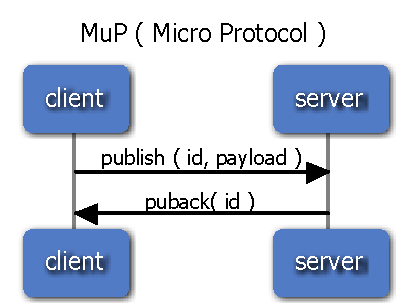
\includegraphics[width=1.0\textwidth]{slides/MuP.pdf}}
   \end{column}
   \begin{column}{0.5\textwidth}
      \begin{itemize}[<+->]
         \item Let's create simple protocol
         \item Simple enough to send payloads
         \item But powerfull enough to make sure it's delivered at least once
         \item Yes it's a small fraction of MQTT
      \end{itemize}
    \end{column}
\end{columns}

\end{frame}

\subsection{Sample protocol}

\begin{frame}{Definition}

  \begin{columns}
      \begin{column}{0.5\textwidth}
        \begin{block}{Header}
          \lstinputlisting[style=customc]{slides/sample_protocol.h}
        \end{block}        
      \end{column}
      \pause
      \begin{column}{0.5\textwidth}
        \begin{block}{Publish/Puback}
          \lstinputlisting[style=customc]{slides/sample_protocol2.h}
        \end{block}
      \end{column}
  \end{columns}
  \pause
  \begin{columns}
      \begin{column}{0.3333\textwidth}
        \begin{block}{Final Structure}
          \lstinputlisting[style=customc]{slides/sample_protocol3.h}
        \end{block}
      \end{column}
  \end{columns}
\end{frame}

\subsection{Usage}

\begin{frame}{Sending}
   \only<1> {
      \begin{columns}
         \begin{column}{1.0\textwidth}
               \begin{block}{Common}
                  \lstinputlisting[style=customc]{slides/sending1.h}
               \end{block}
         \end{column}
      \end{columns}
   }
   \only<2> {
      \begin{columns}   
         \begin{column}{1.0\textwidth}
            \begin{block}{Sending}
               \lstinputlisting[style=customc]{slides/sending2.h}
            \end{block}
         \end{column} 
      \end{columns}   
   }  
\end{frame}

\begin{frame}{Receiving}
   \only<1> {
      \begin{columns}
         \begin{column}{1.0\textwidth}
               \begin{block}{Receiving}
                  \scalebox{0.8} {
                     \lstinputlisting[style=customc]{slides/receiving.h}
                  }
               \end{block}
         \end{column}
      \end{columns}
   }
   \only<2> {
      \begin{columns}
         \begin{column}{1.0\textwidth}
               \begin{block}{Analyse}
                  \lstinputlisting[style=customc]{slides/analyse.h}
               \end{block}
         \end{column}
      \end{columns}
   }   
\end{frame}

\begin{frame}{Conclusions}
   \begin{itemize}[<+->]
      \item Code is long and less readable
      \item This is error prone
         \begin{itemize}[<+->]
            \item Memory leaks
            \item Reordering sequence in wrong way
            \item Level of complication
         \end{itemize}
      \item Order of states may not reflect the real order of execution
   \end{itemize}
\end{frame}

\section{ Coroutines? }

\subsection{ How does it work? }

\begin{frame}{ Implementation }
   \begin{columns}
      \begin{column}{0.5\textwidth}
         \begin{block}{Coroutine macros}
            \scalebox{0.8} {
               \lstinputlisting[style=customc]{slides/impl.h}
            }
         \end{block}
      \end{column}
      \begin{column}{0.5\textwidth}
         \begin{block}{Cons}
            \begin{itemize}[<+->]
               \item Can't use switch inside coroutine
               \item Requires passing the coroutine state
               \item Requires to declare all variables before the coroutine
               \item Requires to re-initialize all variables on every re-entry
            \end{itemize}
         \end{block}
      \end{column}
   \end{columns}
\end{frame}

\begin{frame}{Sequence of operations for sending/receiving MuP}
   \begin{columns}
      \begin{column}{0.5\textwidth}
         \begin{block}<1->{Init and send}
            \centerline{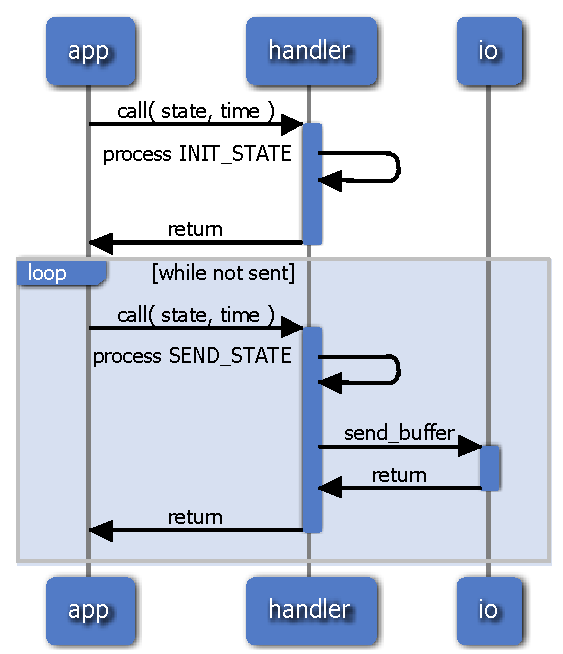
\includegraphics[height=0.5\textheight]{slides/send_recv.pdf}}
         \end{block}
      \end{column}
      \begin{column}{0.5\textwidth}
         \begin{block}<1->{Receive and analyse}
            \centerline{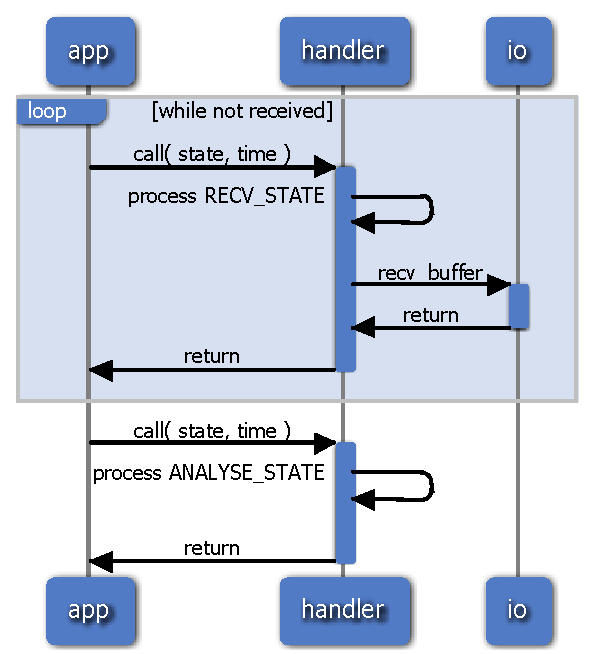
\includegraphics[height=0.5\textheight]{slides/send_recv2.pdf}}
         \end{block}
      \end{column}
   \end{columns}
   \begin{columns}
      \begin{column}{1.0\textwidth}
         \begin{scriptsize}
            \begin{itemize}[<+->]
               \item We are able to execute some part of the code but than we have to wait for the next iteration
               \item We prereserve the state of processing between each execution
               \item We enter to the proper place using switch
            \end{itemize}
         \end{scriptsize}
      \end{column}
   \end{columns}
\end{frame}

\subsection{ How it can be converted? }

\begin{frame}{ Solution ? }
      \begin{block}{Coroutine}
         \scalebox{0.65} {
            \lstinputlisting[style=customc]{slides/coroutines.h}
         }
      \end{block}
\end{frame}

\subsection { Coroutine code analysis }

\begin{frame} { Coroutine analysis - sending }
   \begin{block}{ sending }
      \scalebox{1.0} {
         \lstinputlisting[style=customc]{slides/coro1.h}
      }
   \end{block}
\end{frame}

\begin{frame} { Coroutine analysis - timeout }
   \begin{block}{ timeout }
      \scalebox{1.0} {
         \lstinputlisting[style=customc]{slides/coro2.h}
      }
   \end{block}
\end{frame}

\begin{frame} { Coroutine analysis - receiving }
   \begin{block}{ receiving }
      \scalebox{1.0} {
         \lstinputlisting[style=customc]{slides/coro3.h}
      }
   \end{block}
\end{frame}

\begin{frame} { Coroutine analysis - analyse }
   \begin{block}{ analyse }
      \scalebox{1.0} {
         \lstinputlisting[style=customc]{slides/coro4.h}
      }
   \end{block}
\end{frame}

\section{ LibXively Coroutines }

\subsection{ MQTT protocol sending analysis }

\begin{frame}{ MQTT sending with coroutines }
   \begin{columns}
      \begin{column}{0.5\textwidth}
         \begin{block}{protocol logic level}
            \centerline{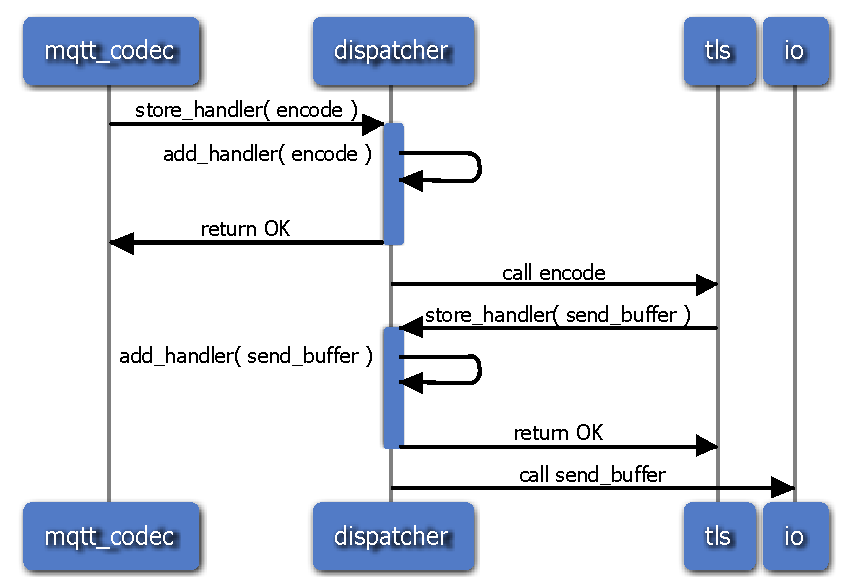
\includegraphics[width=1.0\textwidth]{slides/mqtt_coroutines.pdf}}
         \end{block}
      \end{column}
      \begin{column}{0.5\textwidth}
         \begin{block}{io logic level}
            \centerline{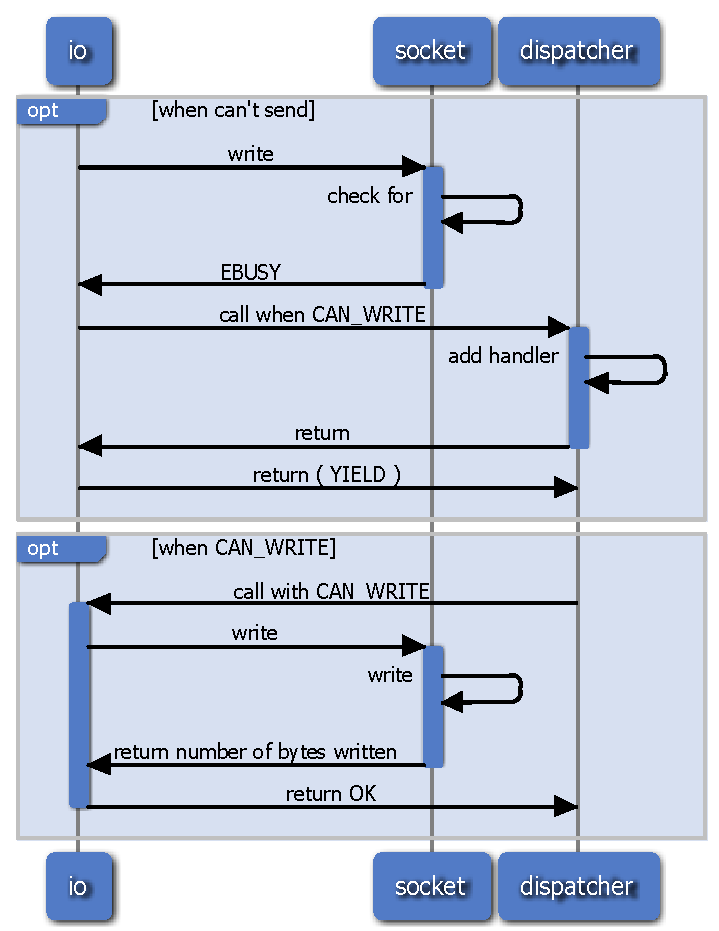
\includegraphics[width=0.8\textwidth]{slides/coroutines_write.pdf}}
         \end{block}
      \end{column}
   \end{columns}
\end{frame}

\section{ Event dispatcher }

\begin{frame} { Reactor pattern sequence diagram }
   \centerline{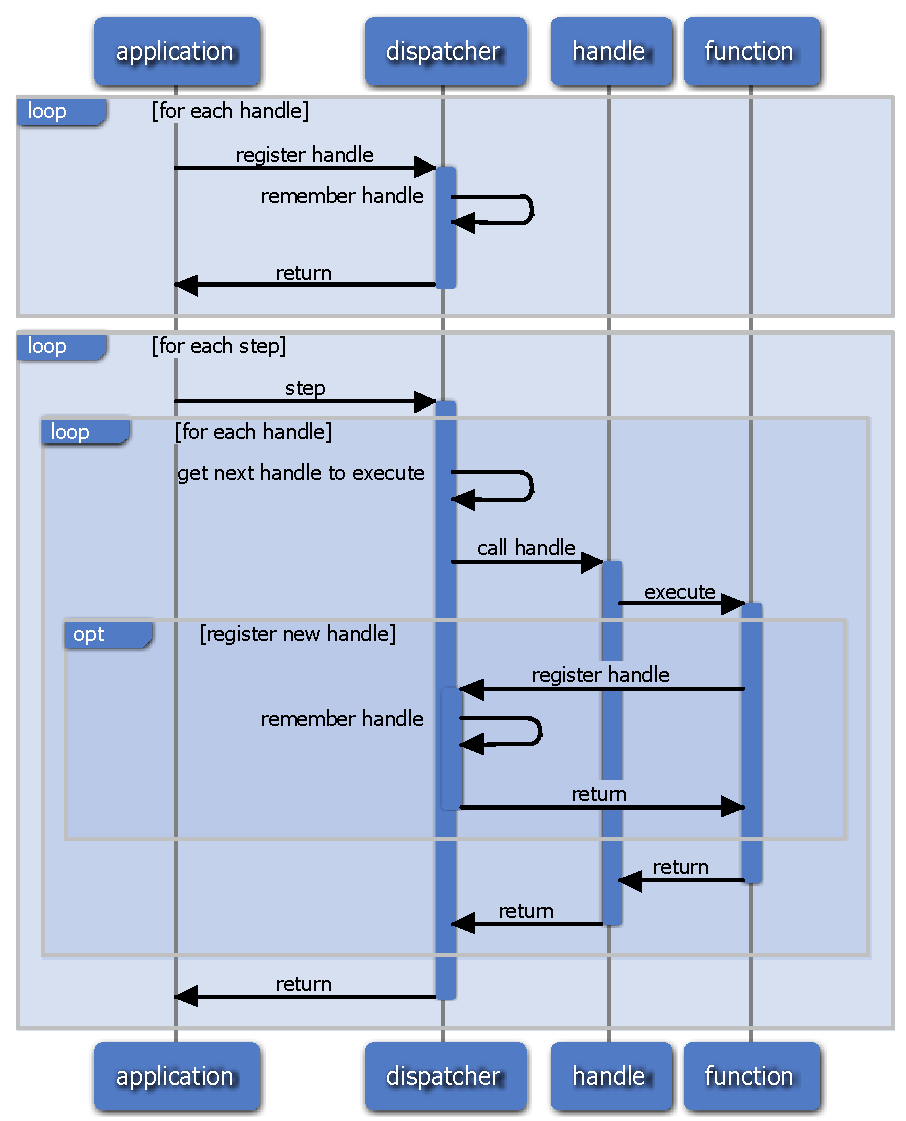
\includegraphics[height=0.9\textheight]{slides/reactor.pdf}}
\end{frame}

\subsection{ Dispatcher Pros \& Cons }
\begin{frame}
   \begin{itemize}[<+->]
      \item Pros
      \begin{itemize}
         \item Separates application specific code from the dispatcher implementation
         \item Increases code reusablity and allows the code to be modular and well splitted 
         \item Allows some simple coarse-grain concurrency while not adding the complexity of multiple threads to the system  
      \end{itemize}
      \item Cons
      \begin{itemize}
         \item The reactor pattern can be more difficult to debug due to the inverted flow of control
         \item By only calling request handlers synchronously, the reactor pattern limits maximum concurrency ( can be replaced with proactor that does not have that limitation )
      \end{itemize}
   \end{itemize}
\end{frame}

\subsection{ LibXively dispatcher responsibilities and flow }
% diagram of LibXively's dispatcher sequence and description of responsibilities
\begin{frame}{ LibXively dispatcher capabilities }
   \begin{itemize}[<+->]
      \item Execute handle at the desired time
      \item Execute handle in a desired order
      \item Execute handle whenever desired event appear on a socket
   \end{itemize}
\end{frame}

\begin{frame}{ Timed events }
   \centerline{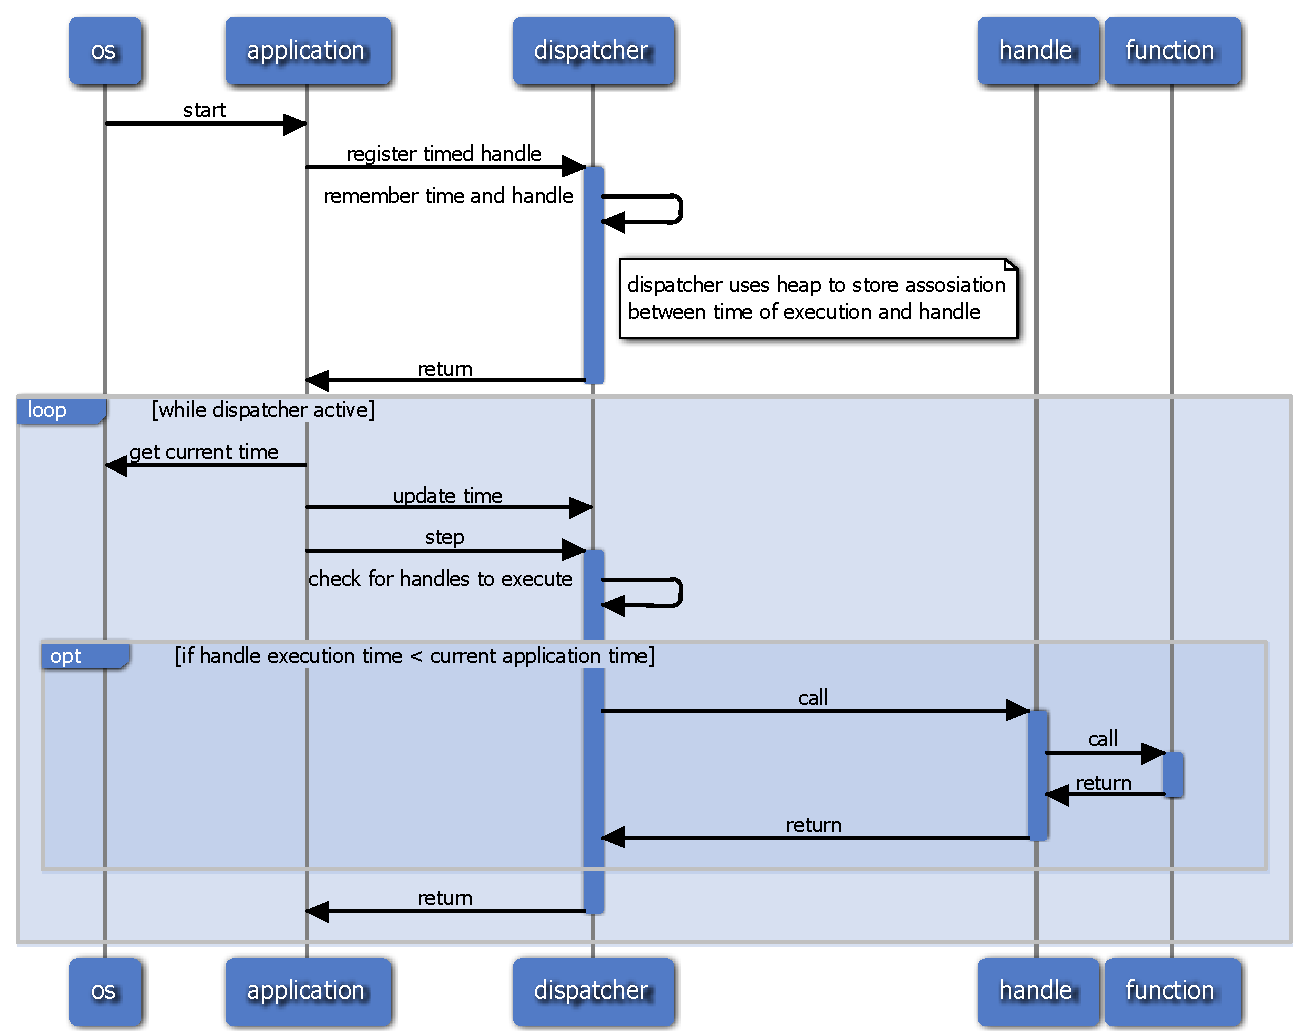
\includegraphics[height=0.9\textheight]{slides/timed_handles.pdf}}
\end{frame}

\begin{frame}{ Queued events }
   \centerline{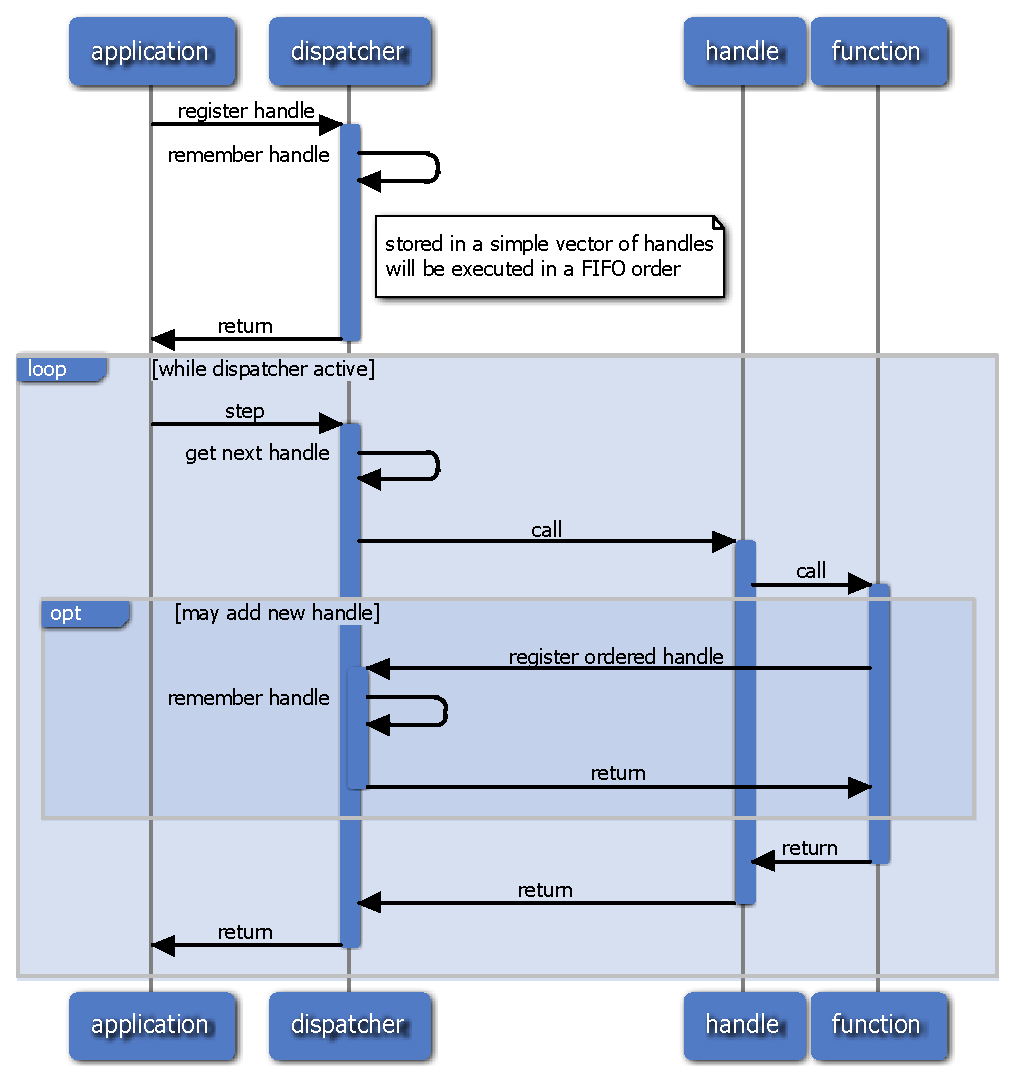
\includegraphics[height=0.9\textheight]{slides/queued_handles.pdf}}
\end{frame}

\begin{frame}{ Socket events }
   \centerline{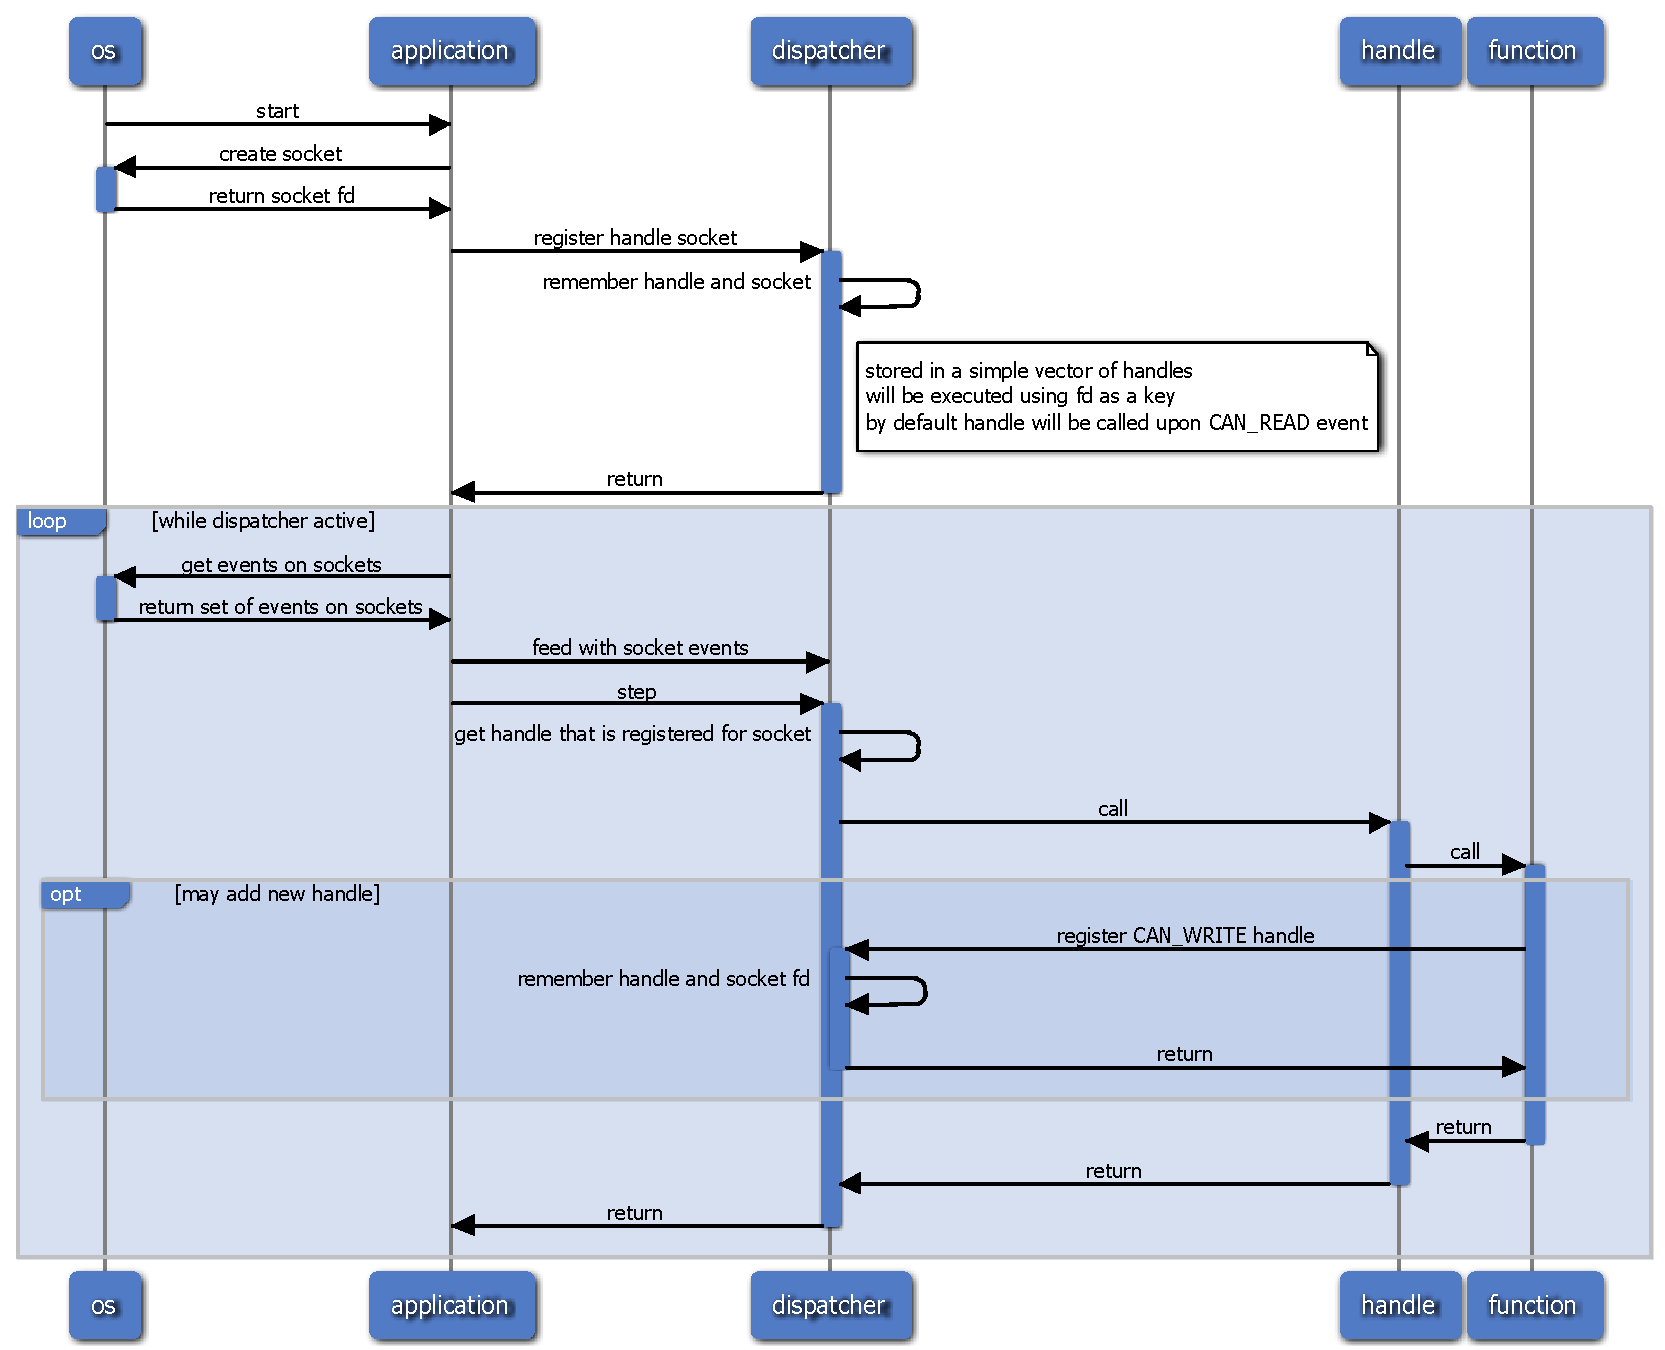
\includegraphics[height=0.9\textheight]{slides/socket_handles.pdf}}
\end{frame}

\subsection{ Usage of LibXively event dispatcher on receiving example }

\begin{frame}{ Processing of event }
   \centerline{\includegraphics[height=0.9\textheight]{slides/dispatcher_sequence.pdf}}
\end{frame}

\section{ The End }

\subsection{ Thank you! }

\begin{frame}{Questions?}
   Questions?
\end{frame}

\end{document}
